\section{Implementation}
% 
In the the prototype, we use the architecture described in Figure \ref{fig:arch-ver2-tech} as the basics for our system design. The idea of the project -- to exchange cryptocurrencies -- is too broad to be implemented without further refinements. To be able to implement the prototype, we need to break this idea down to a list of desired functions or functional requirements. Furthermore, the idea of this product includes some overall themes that the solution should follow, such as security and decentralisation. These \textit{themes} can be broken down to Non-functional requirements \acrshort{nfr}, which describe properties of the system. The further implementation work needs to consider these \acrshort{nfr}s.

\subsection{Prototype requirements}

In this section, we will describe the desired behaviour of the prototype using functional and non-functional requirements. In the first part, functional requirements are used to describe the intended functionality of the system as a whole, as seen from user's perspective. In the second part, we will capture some important characteristics that the system should have, using non-functional requirements.

\subsubsection{Functional requirements}
Usually, functional requirements would come from the users of the system, product owner and other stakeholders. In this project, the authors took the role of the product owner and envisioned the first set of requirements. This first set made up the prototype requirements. In further releases, users and other stakeholders would likely need to be considered.

% we list the requirements for the prototype, so that the idea can be demonstrated clearly. Requirements necessary for demonstrating the idea were prioritised, the others were not worked upon. We ranked the requirements by their importance and then sorted them in a MoSCoW table. We used this table to prioritise the areas for implementation. In a market-ready product, many requirements would most likely be different.

The idea of the system is to allow users trade Ether for another cryptocurrency, which is Bitcoin in this case. Both the user that sells Ether and buys Bitcoin (in previous chapter also referred to as \textit{Alice}) and the user that buys Ether and sells Bitcoin (previously referred to as \textit{Bob}) interact with the same application. For clarity, for the rest of this chapter, we will refer to the Ether selling user as \textit{primary user} and their trading partner (Ether buying user) as \textit{secondary user}.

The requirements for the prototype were selected in such way, so that the overall idea of the system can be demonstrated. The selection is demonstrated in Table \ref{tab:pt-func-reqs}. 

\begin{table}[ht]
    \centering
    \begin{tabularx}{\textwidth}{|l|X|}
    \hline
    \textbf{Requirement ID}& \textbf{Requirement text}\\
    \hline
    PT-FR-1 & The primary user and the secondary user should be able to agree on the terms of the transaction.\\
    PT-FR-2 & The primary user must be able to deploy a smart contract to the Ethereum network.\\
    PT-FR-3 & The secondary user should be able to verify contract deployment.\\
    PT-FR-4 & The secondary user should be able to transfer Bitcoin.\\
    PT-FR-5 & In case secondary user does not transfer Bitcoin, primary user must receive their Ether back.\\
    \hline
    \end{tabularx}
    \caption{Initial set of functional requirements on the prototype.}
    \label{tab:pt-func-reqs}
    \end{table}

% 
\subsubsection{Non-functional requirements}
The overall goal is to develop a secure solution, that does not allow a malicious actor to gain control over other users' funds. To achieve this, the architecture envisioned in Figure \ref{fig:arch-ver2-tech} (p. \pageref{fig:arch-ver2-tech} should be used to carry out the transaction. Furthermore,centralisation the system should be avoided, so that the users can continue using the system even if any particular provider goes offline or is attacked. Table \ref{tab:pt-func-reqs} lists these non-functional requirements.

\begin{table}[ht]
    \centering
    \begin{tabularx}{\textwidth}{|l|X|}
    \hline
    \textbf{Requirement ID}&\textbf{Requirement text}\\
    PT-NFR-1 & The system must implement architecture proposed in Figure \ref{fig:arch-ver2-tech} (p. \pageref{fig:arch-ver2-tech}.\\
    PT-NFR-2 & There should not be single point of failure in the system.\\
    PT-NFR-3 & No other party should have control over the funds of primary user and secondary user.\\
    PT-NFR-4 & Primary user and secondary user must be ably to verify the status of their transaction.\\
    \hline
    \end{tabularx}
    \caption{Non-functional requirements drawn from the initial idea.}
    \label{tab:pt-nonfunc-reqs}
\end{table}

The design of the final architecture, described in the following section is based on these functional and non-functional requirements. The design of the individual system components also takes these requirements into consideration and uses them to derive individual requirements for each component.

%%%%%%%%%%%%%%%%%%%%%%%%%%%%%%%%%%%%%%%%%%%%%%%%%%%%%%%%%%%%%%%%%%%%%%%

% Using FR to describe how the system will operate
 
% begin by FR of the prototype: what functions are included? what parts of the idea are "business critical" - contract deployment
% what it must do
% what it might do
% what it won't do (but should be in the market ready version)

% then NFR of the prototype: how does the system behave
% reqs - no single Point of failure
% reqs - no "last minute pull outs" - once transaction is made, it is final
% reqs - security - 3rd party cannot steal funds if part of the system fails
% reqs - transparency - users need to be able to verify the process


% % Then:
% % each component:
% % Functional reqs: what it does

% % Non-functional reqs - how does it help to achieve the overall NFRs

% //Overall requirements

% //HERE: MoSCoW with requirements (probably?)
% //Maybe: detailed requirements for each component separately

\subsection{System components}
The proposed system consists of several components that interact together. As per requirement PT-NFR-1, the system needs to follow the architecture described in \ref{fig:arch-ver2} (p. \pageref{fig:arch-ver2}). The the main point of user interaction for both primary user and secondary user is the system front end. The front end communicates with Ethereum blockchain via Ethereum node, to deploy a custom smart contract, which operates logic described in figure \ref{fig:simple-logic} (p. \pageref{fig:simple-logic}) and with a back end acts as a communication channel\footnotemark between users. To operate its logic, the smart contract communicates with an oracle. The oracle queries a blockchain explorer provider to learn about the status of a transaction and sends the updates back to the smart contract. User triggers the events in the Android application and validates events on the blockchain. The validation should be done with use of other systems than the Android application itself. Figure \ref{fig:system-overview} depicts the system parts and their relations.

\footnotetext{In the previous examples, we have always considered that the two trading parties -- Alice and Bob agreed on the terms of the transaction beforehand using a separate channel. For this prototype, we have decided to include a communication channel, to enable users interact and agree on the transaction terms within the prototype. While this functionality is certainly not novel, nor it is the focus of this project, it complements the prototype and showcases, how it could be used in real-world.}

\begin{figure}[p]
    \centering
    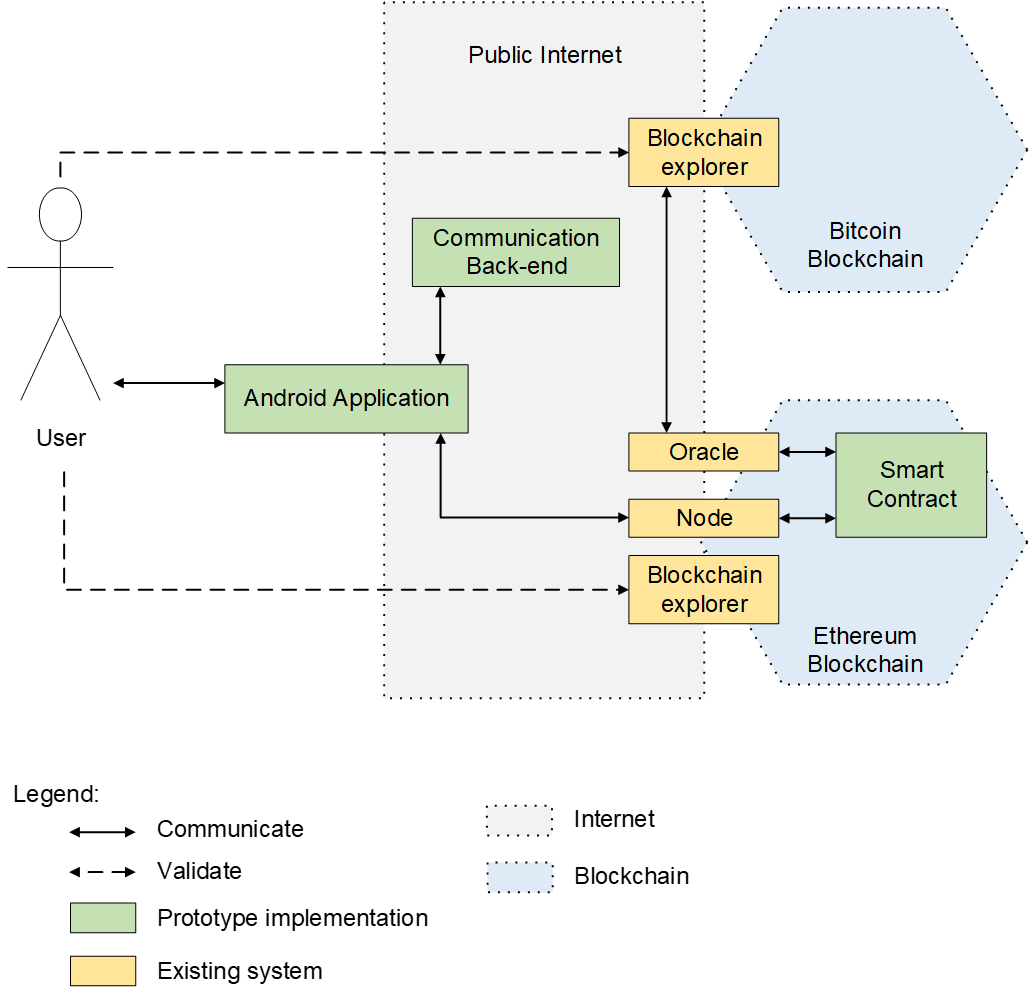
\includegraphics[width=\textwidth]{system-overview}
    \caption[itemize]{
    Overview of the system parts:
    \begin{enumerate*}[label=(\roman*)]
        \item \textit{User} communicates directly with the Android application and verifies data on the blockchain.
        \item \textit{Android application} fetches data about existing offers from the communication back-end and sends new smart contracts to the Ethereum node.
        \item \textit{Node} communicates with other nodes in the Ethereum network, maintains the status of the blockchain and deploys new smart contracts to the network.
        \item \textit{Smart contract} contacts oracle after deployment and holds the funds until the oracle has cleared the transaction as approved.
        \item The \textit{oracle} queries the Bitcoin block explorer to learn about the status of the transaction and communicates the result back to the smart contract.
    \end{enumerate*}
    }
    \label{fig:system-overview}
\end{figure}

\subsection{Requirements of system components}

//INTRO?

\subsubsection{Application front end}
The front end part of the proposed system has the task of receiving user's input and presenting the progress of a deployed transaction. It communicates directly with the node in order to deploy smart contracts and receive account balance and transaction hashes. Application receives data from the user (such as transaction value or destination address), verifies their validity and prepares the data in a format that can be consumed by the node. Front end also contacts the node and presents eventual replies to the user in an user-comprehensible format. If a reply is not received, the application needs to notify the user too.

\begin{figure}[ht]
    \begin{framed}
    \begin{tabular}{l l}
        \multicolumn{2}{c}{\textbf{Functional requirements}}\\
        \textbf{Requirement AF-1}&Verify user input.\\
        \textbf{Requirement AF-2}&Convert user input into node-compatible format.\\
        \textbf{Requirement AF-3a}&Deploy contract to the node.\\
        \textbf{Requirement AF-3b}&Query node for address balance.\\
        \textbf{Requirement AF-3c}&Query node for address nonce.\\
        \textbf{Requirement AF-4}&Display response from the node.\\
        
        \multicolumn{2}{c}{\textbf{Non-functional requirements}}
    \end{tabular}
    \end{framed}
   
    \caption{Caption}
    \label{fig:my_label}
\end{figure}

\subsubsection{Ethereum Node}
Ethereum node plays vital role in the application, as it deploys smart contracts, created by the user to the Ethereum network. If a node fails to do that, users cannot use the application for its purpose. We can say that the role of the node is \textit{business critical}.

The node needs to send transactions to the Ethereum network reliably and without delay. When queried, it must provide accurate and most up-to-date response. We can refer to these goals as trustworthiness and reliability. Since it is impossible to guarantee trustworthiness and reliability of any single node controlled by a third party, it would be in user’s best interest to operate their own node. However, operating a full node requires resources which may not be available on a mobile device.

If conditions do not allow for operation of a full node, second best alternative would be to query multiple nodes with the same request and accept the most common answer as the correct one. Since it is safe to suppose that majority of the nodes in the network are honest nodes, this would prevent single malicious node from affecting or halting the transaction process and would also resolve problems caused by downtime of any particular node. While this architecture certainly can be achieved, it is complex to fully implement such a scheme. The requirements 

\begin{figure}[ht]
    \begin{framed}
    \begin{tabular}{l l}
        \textbf{Requirement EN-1}&Send transactions to the network.\\
        
    \end{tabular}
    \end{framed}
   
    \caption{Caption}
    \label{fig:my_label}
\end{figure}

The consequences of nodes not fulfilling these requirements could be the impossibility to retrieve wallet balance and the impossibility to deploy contracts to the network, which would result in users not being able to use the application. Since the transaction for contract deployment is singed on user’s device, the node cannot alter transactions it receives. If user deployed a contract, but the node refused to provide transaction hash of this transaction, user’s trading partner would never transfer the second currency. The user would therefore waste funds on paying for the gas for the contract deployment, but would not lose funds as these would be transferred back after the contract timeout period has elapsed. //EXPLAIN ABOUT THIS/REFER TO EXPLANATION

\subsubsection{Smart contract}
The smart contract should implement the logic described in //DESCRIBED WHERE. It also must emit an event after construction as it is necessary for the user’s trading partner to verify that the contract was deployed as agreed. For its correct execution, it must also cater for any costs required to cover the services of an oracle. Application should reflect such costs in user interface, if this is the case.

Optionally, the contract can also emit an event when it receives a response from the oracle. If a transaction was not completed, such event could help users understand the reason.

Contracts should also be as short as possible to keep the costs of deployment and operation of the contract to minimum, as the user needs to pay for gas for every bytecode instruction. High prices of operating a contract could deter users from using the application.


\subsection{Implementation of system components}

//DUNNO? Section intro I suppose

\subsubsection{Application front end} 

To implement this functionality //functionality mentioned in XXX, the Android platform was chosen. Currently, it is the most used operating system in the world\footnotemark which ensures compatibility with significant number of devices. It is capable of carrying out the tasks outlined above and it does not require a centralised server to operate (as opposed to a website/web application). Development tools and documentation available free of charge and author's previous knowledge of Android programming were the further supporting arguments for Android. Android \acrshort{api} version 26 (Android Oreo) was chosen, as it is the newest supported version at the time of writing, although this has little practical implications. The prototype uses some user-interface features that were first introduced in \acrshort{api} version 22, so the minimal required Android version could be rolled back to this version without any changes.
% 
\footnotetext{\url{http://gs.statcounter.com/os-market-share}, as of 06-05-2018. See //REFERENCE TO APPENDIX for details}

In conjunction with Android, standard Java programming language was used. This is as opposed to Kotlin, a statically typed programming language, which was developed by JetBrains\footnotemark and pronounced the official Android programming language by Google on 17th May 2017 \cite{Vasic2017MasteringKotlin}. 
% 
\footnotetext{JetBrains is a company that created IntelliJ and other popular \acrshort{ide}s. \url{https://www.jetbrains.com/}}
% 
Many industry professionals suggest migrating to Kotlin as it offers several advantages \cite{Vasic2017MasteringKotlin} \footnotemark, but it has no direct implication on the prototype, as it compiles to the same byte-code as Java.
% 
\footnotetext{\url{https://medium.com/@magnus.chatt/why-you-should-totally-switch-to-kotlin-c7bbde9e10d5}, accessed 06-05-2018}

We will describe the structure of the prototype using the terminology of the \acrfull{modelvp} architecture pattern, which describe the architecture of an application in three layers or interfaces:
\begin{enumerate*}[label=(\roman*)]
    \item \textit{Model}
    \item \textit{View} and
    \item \textit{Presenter}
\end{enumerate*}.
The prototype does not fully succeed in following this patter, but it does share the major features with it. In the prototype, the split between model and presenter is not ideal and these two layers partially overlap. The approximation is as follows:
\begin{itemize}[noitemsep]
    \item Fragments have the role of the \textit{view} part
    \item \texttt{MainActivity} and wrapper classes have the role of the \textit{presenter} part
    \item \texttt{TradeDeal} and \texttt{BtcOffer} have the role of the \textit{model}.
\end{itemize}

\paragraph{View} The view part of the \acrshort{modelvp} is represented by eight fragment classes. Each fragment represents one screen of the application. XML files are used to describe the user interface elements of each fragment. Fragments read user inputs from these elements and update them accordingly with information recieved from \textit{presenter} interface. Example of such fragment is \texttt{DeployContractFragment}, which displays wallet balance in one \texttt{TextView} and reads user's input from another.

\paragraph{Presenter} 
\begin{sloppypar}
To navigate between fragments and update the view with new data, \texttt{MainActivity} is used. It implements interface \texttt{OnFragmentInteractionListener} that listens for user interaction in the fragments and responds accordingly. For example if the user selects to create a new offer by clicking on appropriate button, fragment calls the \texttt{onFragmentInteraction} method of \texttt{OnFragmentInteractionListener}, which is implemented in the activity class. \texttt{MainActivity} then initiates fragment transaction and replaces the old fragment with \texttt{CreateOfferFragment}.

The \textit{presenter} part of \acrshort{modelvp} is further complemented by three wrapper classes (\texttt{EthereumWrapper}, \texttt{BitcoinWrapper} and \texttt{FirebaseWrapper}). These classes contain methods to convert data to and from user-comprehensible format (e.g. method \texttt{satoshiToBtcString} from \texttt{BitcoinWrapper} class that converts the amount in satoshi to more user-friendly format -- decimal Bitcoins) and to communicate with the network (e.g. method \texttt{fetchExistingOffers} in \texttt{FirebaseWrapper} to get data from the database or method \texttt{sendContract} in \texttt{EthereumWrapper} to deploy contract to the network).
\end{sloppypar}

\paragraph{Model}
The \textit{model} interface in the prototype is represented by classes \texttt{BtcOffer} and \texttt{TradaDeal}. The first is used to contain all details of an offer to sell Bitcoins, both when a new offer is created and when existing offers are loaded from the database. When a user decides to proceed with an offer, \texttt{BtcOffer} is transformed into a \texttt{TradeDeal}. Trade deal holds further details of the offer, such as the deploying address and is used during the transaction validation process and during contract deployment.

The Java representation of the smart contract, \texttt{SmartExchange2} is also part of the model. It does not operate any logic in the Android application, but it holds the binary representation of the compiled Solidity code. The methods of this Java representation would also be used to communicate with an already deployed smart contract, although this functionality is currently not implemented in the prototype as it is not needed. \texttt{SmartExchange2} also contains the constructor used to pass initial value to the contract upon deployment. It is important to note, that \texttt{SmartExchange2} is an auto-generated code by the Web3j library, which takes ABI and BIN files of a compiled contract as the input and returns a single Java class as the output.

\subsubsection{Node}
As mentioned in //REFERENCE TO SECTION OF SOTA, Etherumj could be used to connect to the Ethereum network. However, running a full node on the Android platform may not be a viable solution, due to limitations of mobile devices. These limitations include storage, network bandwidth and power consumption. Fully connected node maintains a local copy of the blockchain (storage) and regularly communicates with the network peers to get the most recent block (network and battery consumption). Alternative solution to lower the load on the mobile device would be to run a light client (//GITHUB REFERENCE), which is targeted specifically for mobile devices and that does not maintain a local copy of the whole blockchain.

To speed up the development, we decided to use a remotely hosted node for this prototype. Instead of deploying own remote Ethereum node, a node-hosting service Infura was chosen. Upon creating an account on Infura’s website, developer is presented with a series of API endpoints – one endpoint for all major Ethereum networks (Mainnet, Kovan, Rynkeby…). Endpoints accept connections from any client and no authentication is needed. This is not an issue, since by design, the prototype signs the transaction on device, before it is deployed to the network, so the node does not have access to any sensitive data.

While running a single node is sufficient to demonstrate the idea of the prototype, more work should be put into implementing the solution with multiple nodes. In a market-ready version of the application, the centralisation implied by using a single node would pose as a major, business critical drawback. This should be one of the first issues to address in any further development of the application.
% 
\subsubsection{Smart Contract}
The contract was written in the Solidity language, as it is currently the recommended (//?) language for smart contracts. The latest available version //SOLIDITY VERSION (probably newest) was used. The smart contract was written using Remix, an in-browser IDE, recommended for use with Solidity, which enables sandbox contract testing. Oraclize (//EXPLAIN WTH IS ORACLIZE) version of Remix was also used to test the functionality of an oracle.

Smart contract in Solidty was then compiled into binary and ABI (//EXPLAIN WHHAT THIS) files, using the solc compiler. The BIN and ABI files where then used by Web3j command line tools to generate Java representation of the Smart contract (//LINK TO FILE IN ATTACHMENT/APPENDIX). On top of the compiled smart contract in binary form, this Java file also includes wrapper methods to invoke the custom constructor and the methods of the contract.

% 
\subsubsection{Oracle}

Using Oraclize for this service... why? Why not?
% 
\subsubsection{Blockchain explorer}
Using blockchain.info... why? Why not?

\subsubsection{Database //Firebase}
The back end for user communication is mostly included in the prototype to demonstrate the flow of the transaction. While in the prototype implementation, the communication back-end is necessary to coordinate actions of primary and secondary user, in a market-ready product it should only play supportive role -- so that even when the back-end is not operational, the application still can be used.


\paragraph{Drawbacks}
Using 1 node in the prototype

Using oraclize in the prototype

Using blockchain.info in the prortytype

Using unsecured database in the prototype.





\subsubsection{Flows/usage}
% 
In this section we will showcase how the app is used - what data is entered when, what screens are presented -- not sure how important is to have this.


